\chapter{بازیابی وفقی سیگنال دیکشنری-تنک با استفاده از نمونه‌برداری تک بیتی}
\label{ch:main}
\newpage
\section{تحلیل سیگنال‌های دیکشنری-تنک}
تا این قسمت از پایان‌نامه به تحلیل و بررسی روش‌های نمونه‌برداری و بازیابی سیگنال‌های تنک پرداخته شده است. در بسیاری از کاربرد‌های عملی، سیگنال مورد بررسی مستقیما و یا در یک دسته از پایه‌های متعامد تنک نیست. در این حالت سیگنال، در یک دیکشنری غیر متعامد تنک خواهد بود.

در ادامه، سیگنال تنک را با
$ \bm{x}\in \R^N $
و دیکشنری افزونه
\LTRfootnote{Redundant}
را با 
$ \bm{D}\in \R^{n\times N} $
نشان می‌دهیم. همچنین سیگنال مورد بررسی با
$ \bm{f}\in \R^n $
 نشان داده شده که به صورت
 $ \bm{f}=\bm{D}\bm{x} $
 با پایه‌های تنک در ارتباط است. مقدار همبستگی ماتریس 
 $\bm{D}$
 به صورت زیر تعریف می‌گردد.
\begin{align}
\label{eq:eq25}
\mu := \max_{1\leq i\neq j\leq N} \dfrac{| \langle d_{i},d_{j}\rangle|}{\norm{d_{i}}_{2}\norm{d_{j}}_{2}}
\end{align}

در رابطه‌ی
\eqref{eq:eq25}
، 
$ d_{i} $
و
$ d_{j} $
نشان‌گر ستون‌های
$i$ام
و
$j$ام
از ماتریس 
$ \bm{D} $
هستند. در صورتی که مقدار
$ \mu = \mu\left(\bm{D}\right) $
کوچک باشد، دیکشنری 
$ \bm{D} $
ناهمدوس
\LTRfootnote{Incoherent}
نامیده می‌شود. با فرض
$ \bm{D} $
به صورت یک ماتریس مربعی با همبستگی پایین، حاصل‌ضرب 
$ \bm{A}\bm{D} $
گوسی است و نتایج حسگری فشرده بازیابی صحیح با استفاده از نمونه‌های
$ \bm{y}=\bm{A}\bm{f}=\bm{A}\bm{D}\bm{x} $
را تضمین می‌کند، در صورتی هدف از این گزارش سیگنال‌های تنک در دیکشنری افزونه است.

در ادامه، به صورت خلاصه دو ساختار مشابه ولی از دو کلاس متفاوت از سیگنال‌های دیکشنری تنک بررسی شده است. این دو کلاس از سیگنال‌ها، تنک-تحلیلی
\LTRfootnote{Analysis-sparse}
و تنک-ترکیبی
\LTRfootnote{Synthesis-sparse}
نامیده می‌شوند. مفاهیم اساسی سیگنال‌های تنک-تحلیلی
و  تنک-ترکیبی
در مراجع
\cite{elad2007analysis,Candes2011,nam2013cosparse}
بیان شده است. در اینجا ما تنها یک مرور خلاصه بر ایده‌ی اصلی می‌کنیم.
\begin{itemize}
\item{
سیگنال
\textbf{تنک-ترکیبی}:

برای ساخت این دسته از سیگنال‌ها، ابتدا، 
$s$
ستون (اتم) از دیکشنری 
$\bm{D}$
، به صورت تصادفی انتخاب می‌گردد (توجه داشته باشید که مجموعه‌ی اندیس‌ها با 
$ T $
نشان داده شده است.). در ادامه مقادیر دامنه‌ی 
$ s $
مولفه از بردار
$ \bm{x} $
به صورت تصادفی از یک توزیع (به عنوان مثال توزیع نرمال) انتخاب می‌گردد. سیگنال 
$ s $
-تنک ترکیبی
$ \bm{f} $
، با ضرب دیکشنری 
$\bm{D}$
در بردار 
$ \bm{x} $
به دست می‌آید.
}
\item{
سیگنال
\textbf{تنک-تحلیلی}:

جهت معرفی این دسته از سیگنال‌ها نیاز به بیان مفهوم متمم-تنکی 
\LTRfootnote{Cosparsity}
است. متمم-تنکی بردار
$ \bm{f} $
در اپراتور
$ \bm{\bm{\Omega}}\in \R^{N\times n} $
،‌ برابر با تعداد صفرهای موجود در
$ \bm{\bm{\Omega}}\bm{f} $
است. با استفاده از مفهوم متمم-تنک می‌توان سیگنال‌های تنک-تحلیلی را به عنوان دوگان تنک-ترکیبی مطرح نمود. ماتریس
$ \bm{\bm{\Omega}}\in \R^{N\times n} $
را به عنوان اپراتور تحلیلی
\LTRfootnote{Analysis operator} 
در نظر بگیرید. برای ساخت سیگنال 
$ s $
-تنک تحلیلی، ابتدا 
$l$
سطر از 
$\Omega$
را به صورت تصادفی انتخاب می‌کنیم (توجه داشته باشید که مجموعه‌ی اندیس‌ها با 
$ \Lambda $
نشان داده شده و
$\vert \Lambda \vert = l$
است). در ادامه بردار تصادفی 
$ \bm{x} $
را با درایه‌‌های
\lr{iid}
گوسی تولید می‌کنیم. سیگنال متمم-تنک با تصویر
$ \bm{x} $
بر مکمل متعامد زیرفضای تولید شده توسط 
$ \bm{\bm{\Omega}}_{\Lambda} $
به دست می‌آید. به عبارت ریاضی
\begin{align}
\label{eq:eq26}
\bm{f}= (\bm{I}-\bm{\Omega}^{\ast}_{\Lambda}(\bm{\Omega}_{\Lambda}\bm{\Omega}^{\ast}_{\Lambda})^{-1}\bm{\Omega}_{\Lambda})\bm{x}
\end{align}
در عبارت فوق، 
$ \bm{\bm{\Omega}}_{\Lambda} $
نشان‌دهنده‌ی سطرهایی از 
$ \bm{\Omega} $ 
است که در مجموعه‌ی 
$ \Lambda $
قرار دارند.
}
\end{itemize}

با دقت در تعریف سیگنال تنک-ترکیبی مشخص است که با حذف ستون‌هایی از 
$\bm{D}$
که در
$ T $
قرار دارند، زیرفضای سیگنال تغییر نمی‌کند. از طرف دیگر، در سیگنال‌های تنک-تحلیلی
مجموعه‌ی اندیس‌های متمم-تنک
($ \langle \omega_{i}, \bm{f} \rangle =0,~ i \in \Lambda $)
تعیین کننده‌ی زیرفضای سیگنال هستند.

در حالت کلی زیرفضای سیگنال‌های تنک-تحلیلی و تنک-ترکیبی با یکدیگر متفاوت هستند. با این حال، از میان تمام زیرفضا‌های مدل 
تحلیلی یکی سازنده‌ی زیرفضای  ترکیبی است. با در نظر گرفتن یکسان بودن زیرفضای سازنده‌ی سیگنال‌های
تحلیلی و
ترکیبی، شکل 
\ref{fig12}
فرآیند ساخت و نمونه‌برداری تک-بیتی از یک سیگنال دیکشنری تنک را نشان می‌دهد.

\begin{figure}
\centering
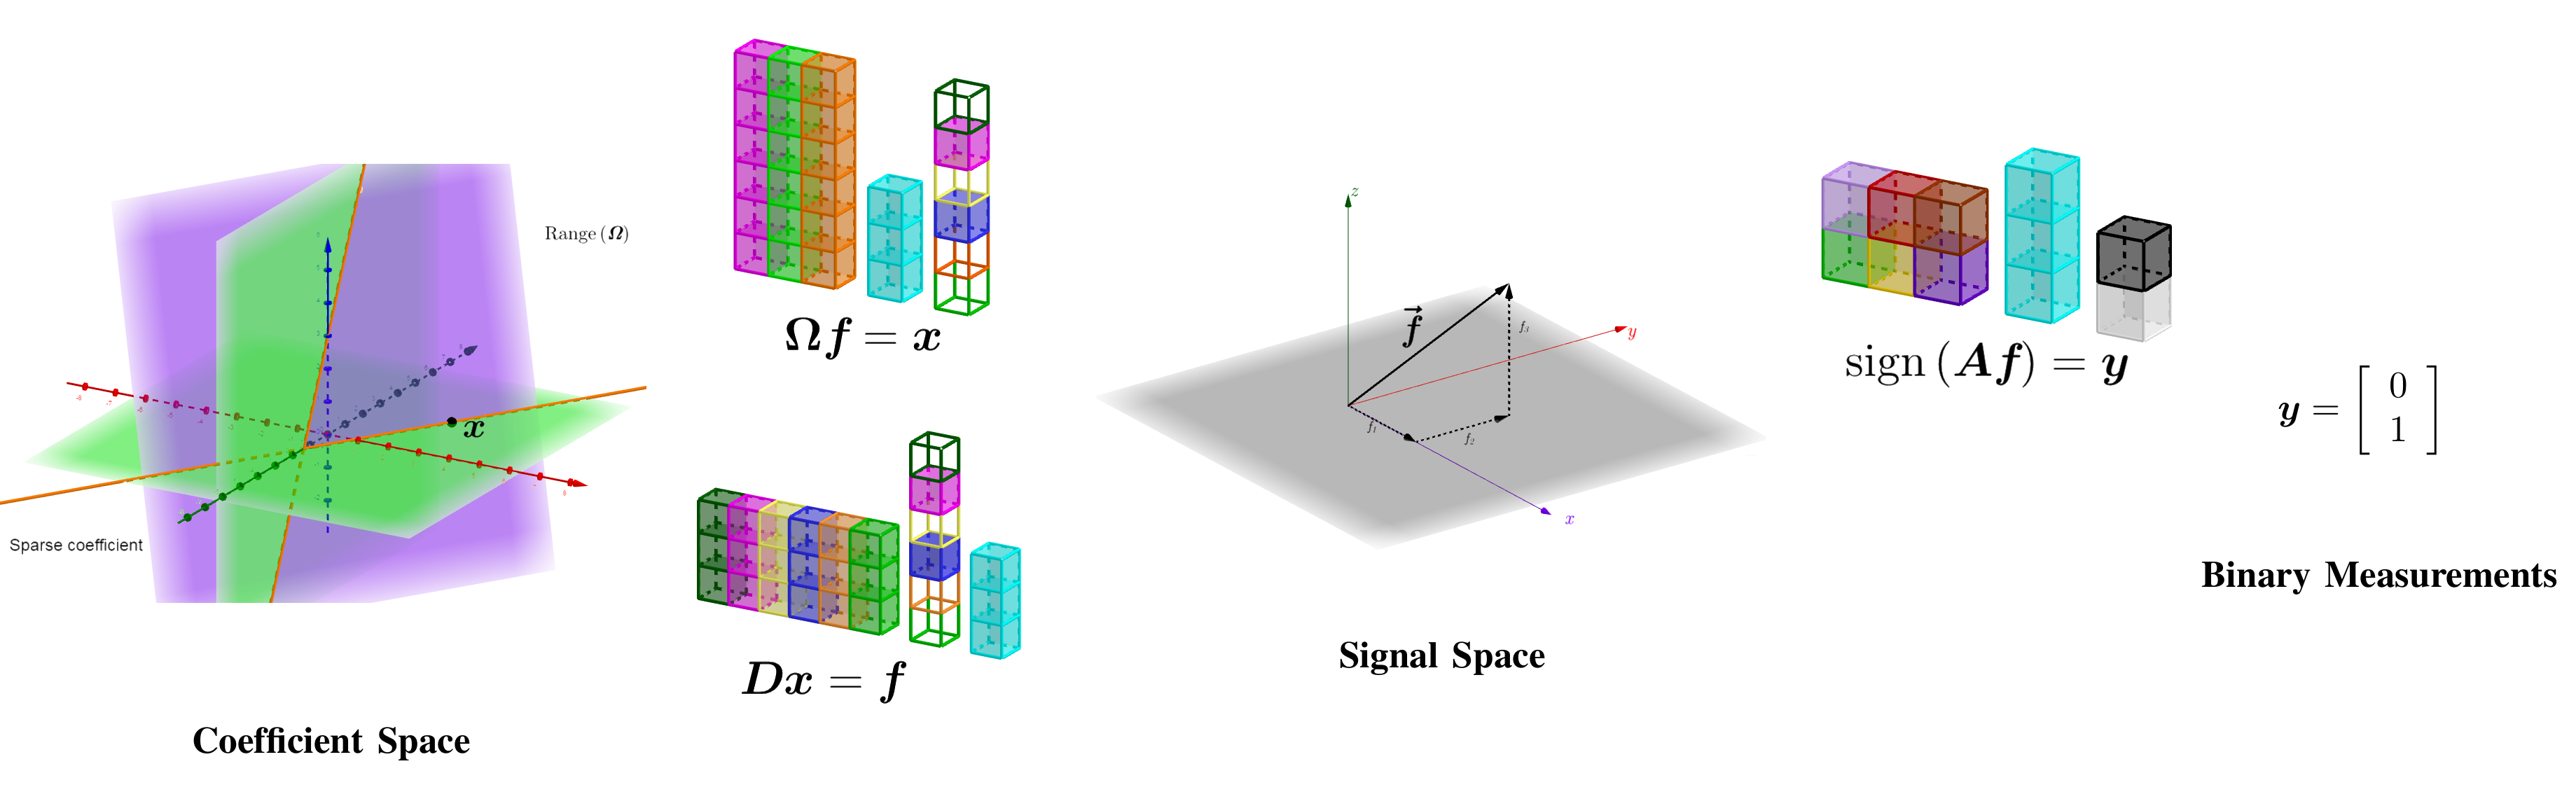
\includegraphics[scale=0.1]{Images/ch3/fig12.png}
\caption{فرآیند ساخت و نمونه‌برداری از یک سیگنال دیکشنری تنک}
\label{fig12}
\end{figure}

در این پایان‌نامه از اپراتور تحلیلی با چارچوب فشرده 
\LTRfootnote{Tight frame}
استفاده شده است. چارچوب فشرده به صورت زیر تعریف می‌گردد.
سطر‌های 
$ \bm{\Omega} $
تشکیل یک چارچوب می‌دهند اگر مقادیر
$ 0< a\leq b < \infty $
وجود داشته باشند، به گونه‌ای که 
\begin{align}
\label{eq:eq27}
a\norm{\bm{f}}^{2}_{2}\leq \norm{\bm{\Omega}\bm{f}}^{2}_{2} \leq b\norm{\bm{f}}^{2}_{2} 
\end{align}
و در صورتی که 
$ a=b $
باشد، 
$ \bm{\Omega} $ 
چارچوب فشرده نامیده می‌شود.


\section{مدل سیستم}
در این بخش مدل سیستم مورد بررسی بیان گردیده است. قبل از بیان مدل، ابتدا چند تعریف مورد استفاده در قسمت‌های بعدی بیان شده است. همچنین در این قسمت تصویر بر نیم‌کره
\LTRfootnote{Hemisphere projection}
ارائه شده است. از این تصویرسازی جهت انتقال مدل نمونه‌برداری 
\eqref{eq:eq11}
به 
\eqref{eq:eq12}
استفاده شده است. همچنین با استفاده از این تصویرسازی، یک اثبات شهودی برای قضیه‌ی اصلی این پایان‌نامه ارائه شده است.
\begin{itemize}
\item{
\textbf{تنکی موثر}\LTRfootnote{Effective sparsity}


نامساوی کوشی-شوارتز مقدار نُرم
$ l_1 $
و 
$ l_2 $
سیگنال 
$ \bm{x}\in \R^{N} $
را به صورت 
$ \norm{\bm{x}}_{1}\leq \sqrt{N}\norm{\bm{x}}_{2} $
با یکدیگر مرتبط می‌کند.
بردار 
$ \bm{x}\in \R^{N} $
$s$-تنک موثر
نامیده می‌شود اگر در شرط زیر صدق کند.
\begin{align}
\label{eq:eq28}
\norm{\bm{x}}_{1}\leq \sqrt{s}\norm{\bm{x}}_{2}
\end{align}
جهت روشن شدن موضوع، مجموعه‌ی تنک موثر
$ \mathcal{K} \in S^{n-1}\cap \sqrt{s}B^{n}_{1} $
را فرض کنید. اگر درجه‌ی تنکی از
$1$
به 
$N$
افزایش یابد، توپ 
$l_1$
از یک چند وجهی محیطی که در ابتدا تنها شامل محورها است، به یک چند وجهی محاطی که شامل 
$ S^{n-1} $
است تبدیل می‌شود. طی این فرآیند با افزایش مقدار
$s$
نقاط اطراف محور‌ها به مجموعه اضافه می‌گردند. جهت نمایش سیگنال‌های 
$s$-تنک
از نماد
$ \Sigma^{N}_{s} $
و برای نمایش سیگنال‌های 
$s$-تنک موثر
از نماد 
$ \Sigma^{N,\text{eff}}_{s} $
استفاده شده است.

اگر سیگنال مورد بررسی از یک دیکشنری تنک انتخاب شده باشد، می‌گوییم که سیگنال
$ \bm{f} $
، 
$ s $
تنک ترکیبی موثر است اگر
$ \bm{f}=\bm{D}\bm{x} $
و برای یک 
$ \bm{x}\in \Sigma^{N,\text{eff}}_{s} $،
$ s $
تنک تحلیلی موثر است اگر
$ \bm{D}^{\ast}\bm{f}\in \Sigma^{N,\text{eff}}_{s} $
باشد.
}
\item{\textbf{مجموعه‌ی پیش-تصویر}
\LTRfootnote{Pre-image set}

برای یک ماتریس (معکوس‌ناپذیر)
$ \bm{D} $
، نماد
$ \bm{D}^{-1}(\mathcal{K}) $
نشان دهنده‌ی مجموعه‌ی پیش-تصویر 
$ \mathcal{K} $
است. به عنوان مثال اگر به ازای
$\bm{f}\in \mathcal{K} $
،
$\bm{f}= \bm{D}\bm{x}$
باشد، آنگاه 
$\bm{x}$
عضو مجموعه‌ی پیش-تصویر 
$\mathcal{K}$
یا
$ (\bm{D}^{\ast})^{-1}(\mathcal{K})$
است.  در موضوع مورد بحث، مجموعه‌ی پیش تصویر
$ \bm{D}^{\ast} $
برای حالت تحلیلی
برابر با
$ \text{Range}(\bm{\Omega}) $
و برای حالت ترکیبی برابر با
$ \text{Span}(\bm{x}) $
است.
}
\end{itemize}

\begin{definition}[تصویر بر نیم‌کره]
\label{defn:HP}
فرض کنید
$ \bm{f}\in \R^{N} $
یک سیگنال اختیاری و
 $ \sigma >0 $
برابر با شعاع نیم‌کره باشد.
سیگنال منتقل شده‌ی
\LTRfootnote{lifted}
$ \bm{f} $
را به صورت
$ \tilde{\bm{f}}:= [\bm{f}^{T}~|~\sigma]^{T}\in \R^{N+1} $ 
تعریف می‌کنیم. تصویر سیگنال انتقال یافته بر نیم‌کره به شعاع
$\sigma$
 به صورت زیر محاسبه می‌گردد.

\begin{align}
\label{eq:eq29}
P_{\sigma}(\tilde{\bm{f}}) =\sigma \dfrac{\tilde{\bm{f}}}{\|\tilde{\bm{f}}\|_{2}}
\end{align}
\end{definition}

\begin{figure}[t]
	\centering
	\begin{subfigure}{0.4\textwidth} % width of left subfigure
		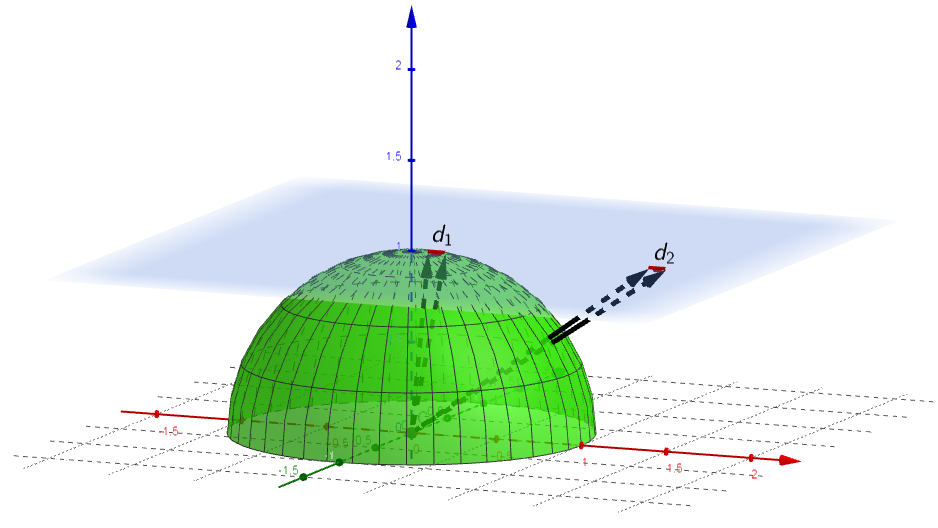
\includegraphics[scale=0.2]{Images/ch3/fig13.png}
		\caption{} % subcaption
		\label{fig13}
	\end{subfigure}
	\vspace{1em} % here you can insert horizontal or vertical space
	\begin{subfigure}{0.4\textwidth} % width of right subfigure
		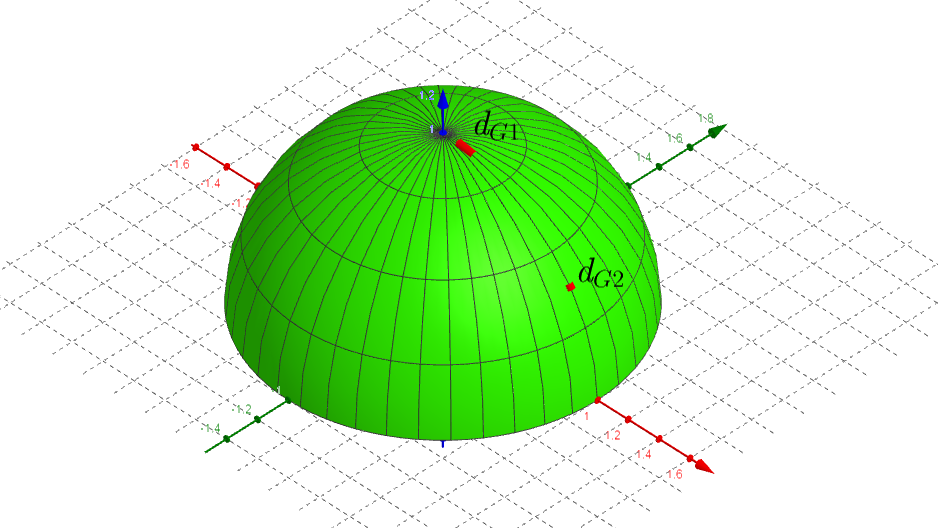
\includegraphics[scale=0.2]{Images/ch3/fig14.png}
		\caption{} % subcaption
		\label{fig14}
	\end{subfigure}
	\caption{تعبیر هندسی تصویر بر نیم‌کره}
\end{figure}

اگرچه تعریف 
\eqref{defn:HP}
بسیار ساده است ولی تعبیر هندسی آن در فهم مساله‌ی ما بسیار موثر است. نکته‌ی بسیار مهم در تعریف
\eqref{defn:HP}
این است که این نگاشت فاصله‌ی بین نقاط را حفظ نمی‌کند. جهت روشن شدن این موضوع به مثال زیر توجه کنید.

فرض کنید 
$ \bm{f}_{1}=[0.1,0,0]^{T} $
،
$ \bm{f}_{2}=[0.2,0,0]^{T} $
،
$ \bm{f}_{3}=[1,0,0]^{T} $
و 
$ \bm{f}_{4}=[1.1,0,0]^{T} $
چهار نقطه از فضای سه بعدی بر روی صفحه‌ی
$ z=1 $
باشند. کاملا واضح است که فاصله‌ی بین 
 $ \bm{f}_{1} $
و
 $ \bm{f}_{2} $
برابر با فاصله‌ی بین
 $ \bm{f}_{3} $
و 
 $ \bm{f}_{4} $
و مساوی با
$ d_{1}=\norm{\bm{f}_{1}-\bm{f}_{2}}_{2}=d_{2}=\norm{\bm{f}_{3}-\bm{f}_{4}}_{2}= 0.1 $
است. در این مثال شعاع نیم‌کره را
$ \sigma =1  $
و مرکز آن را
$ [0,0,0]^{T} $ 
در نظر می‌گیریم (شکل
\ref{fig13}
).
در ادامه نقاط را بر روی نیم‌کره تصویر می‌کنیم (شکل
\ref{fig14}
). فاصله‌ی ژئودزیک بین نقاط تصویر شده به صورت زیر محاسبه می‌گردند.
\begin{align*}
	 d_{G1}&=d_{G}(P_{\sigma}(\tilde{\bm{f}}_{1}),P_{\sigma}(\tilde{\bm{f}}_{2}))= 0.0311\\
	 d_{G2}&=d_{G}(P_{\sigma}(\tilde{\bm{f}}_{3}),P_{\sigma}(\tilde{\bm{f}}_{4}))= 0.0103.
\end{align*}

تفاوت در اندازه‌های تصویر شده با افزایش مقدار نُرم 
$l_2$
افزایش می‌یابد. در کاربرد مورد استفاده‌ی ما با تغییر شعاع نیم‌کره به اندازه‌ی مناسب این تفاوت کنترل شده است.

پس از بیان تعاریف مورد نیاز در قسمت‌های بعدی در این قسمت مدل سیستم بررسی شده است.
فرض کنید، 
$ \bm{f}\in \R^{n} $
یک سیگنال
$s$-تنک ترکیبی
 یا
$s$-تنک تحلیلی
و 
$ \bm{A} $
ماتریس اندازه‌گیری باشد.
بر خلاف روش‌های موجود جهت بازیابی سیگنال‌های دیکشنری-تنک با استفاده از نمونه‌های تک-بیتی که در یک مرحله و با یک تنظیمات تمامی نمونه‌ها را اخذ می‌کند، ما این فرآیند را در چند مرحله انجام می‌دهیم. در این کار آستانه‌ها در طی روند نمونه‌برداری و با استفاده از اطلاعات نمونه‌های قبلی، به صورت وفقی تغییر می‌کند. توجه داشته باشید که ماتریس
$ \bm{A} $
به صورت تصادفی ایجاد شده است ولی در طی روند نمونه‌برداری ثابت فرض می‌شود. همچنین جهت تعریف آستانه‌ها از آستانه‌های ابعاد بالا 
$ \bm{\varphi}^{(i)}\in \R^{n} $
استفاده شده است.
 شکل 
\ref{fig15}
بلوک دیاگرام سیستم مورد بررسی را نشان می‌دهد.
\begin{figure}
	\centering
	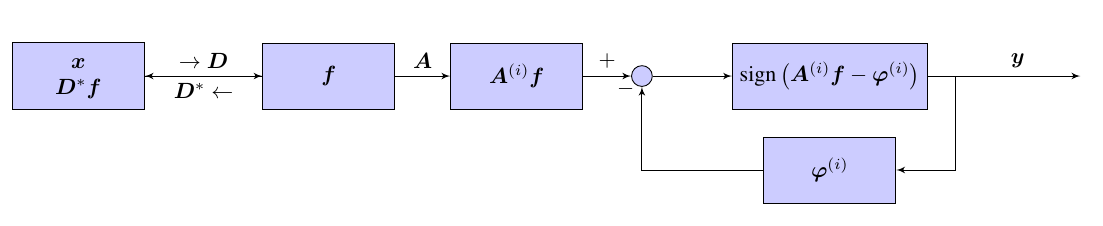
\includegraphics[scale=0.4]{Images/ch3/fig15}
	\caption{بلوک دیاگرام مدل نمونه‌برداری وفقی سیگنال‌های دیکشنری تنک}
	\label{fig15}
\end{figure}

\subsection{بازیابی تک مرحله‌ای}
در روش پیشنهادی، از نتایج به دست آمده در مراحل میانی، جهت بهبود فرآیند وفقی استفاده شده است. در این بخش، هر مرحله از الگوریتم به صورت جداگانه بررسی شده است. هر مرحله از الگوریتم را بازیابی تک مرحله‌ای
\LTRfootnote{Single step recovery}
می‌نامیم. در بازیابی تک مرحله‌ای، در مرحله‌ی 
$i$ام
 ، ماتریس اندازه‌گیری
 $ \bm{A} $
 و آستانه برابر با
 $ \bm{\tau} $
 است.
 قضیه‌ی 
 \ref{theorem:thm8}
 رابطه‌ی بین خطای بازیابی و تعداد نمونه‌ها در بازیابی تک مرحله‌ای را نشان می‌دهد.
 
\begin{theorem}
\label{theorem:thm8}
فرض کنید
$ \epsilon,r,\sigma,C,c^{\prime},\gamma >0 $
و درایه‌های
$ \bm{A}\in \R^{m\times n} $
 از توزیع استاندارد نرمال انتخاب شده باشند. همچنین فرض کنید
 $ \tau_{i}~ i=1,\cdots,m $
 از توزیع گوسی با میانگین صفر و واریانس 
$ \sigma^{2} $
و به صورت مستقل از
$ \bm{A} $
انتخاب شده باشند. با فرض سیگنال
$ \bm{f}\in \R^{n} $
به عنوان یک سیگنال 
$ s $-تنک
تحلیلی(ترکیبی)
در دیکشنری
$\bm{D}\in \R^{n\times N}$
با 
$ \|\bm{f}\|_{2}\leq r $
و
$ \|\bm{D}^{\ast}\bm{f}\|_{1}\leq \sqrt{s} r $
، اگر ما تعداد
$ m \geq C(r/\sigma+\sigma / r)^{6}(r^{2}/\sigma^2+1)\epsilon^{-6}s \log (N/s) $ 
نمونه با استفاده از مدل نمونه‌برداری
\eqref{eq:eq12}
دریافت کنیم، با احتمال حداقل
$ 1-\gamma \exp{(-c^{\prime}m \epsilon^{2} r^2\sigma^2/ (r^2+\sigma^2)^2)} $
پاسخ
\begin{align}
\label{eq:SSR}
 \bm{f}_{\varDelta}~=~\mathop{\arg\min}_{\bm{h}\in \R^{n} } \norm{\bm{D}^{*}\bm{h}}_{1}\quad \text{s.t.} \quad   \bm{y} = \text{sign}\left(\bm{A}\bm{h}-\bm{\tau}\right), \: \norm{\bm{h}}_{2}\leq r,
\end{align}
 در شرط زیر صدق خواهد نمود:
\begin{align}
\|\bm{f}-\bm{f}_{\varDelta}\|_{2}\leq \epsilon r
\end{align}
\end{theorem}
\begin{proof}
اثبات این قضیه در 
\ref{Appndx1}
آورده شده است.
\end{proof}

\section{نتایج اصلی}

\subsection{آستانه‌ی ابعاد بالا}
الگوریتم پیشنهادی جهت تولید آستانه‌های ابعاد بالا در الگوریتم
\ref{alg:HDTG}
آورده شده است. خروجی الگوریتم شامل دو بخش است. بخش اول، یک نقطه‌ی مشخص در فضای سیگنال است که با استفاده از پاسخ تقریبی مرحله‌ی قبل از نمونه‌برداری محاسبه می‌گردد. این نقطه مرکز مجموعه‌ای است که قصد داریم با نمونه‌برداری آن را برش دهیم (در مرحله‌ی اول از الگوریتم این نقطه برابر با مبدا است.). 


\begin{algorithm}
	\caption{$ \Phi $: مولد آستانه در ابعاد بالا}
	\label{alg:HDTG}
	\begin{algorithmic}[1]
		\renewcommand{\algorithmicrequire}{\textbf{ورودی:}}
		\renewcommand{\algorithmicensure}{\textbf{خروجی:}}
		\REQUIRE ماتریس اندازه‌گیری $ \bm{A} $, تعداد نمونه‌ها $ b $, واریانس لغزش‌ها $ \sigma^{2} $, سیگنال تخمینی $ \hat{\bm{f}} $.
		\ENSURE بردار آستانه در ابعاد بالا $\bm{\varphi}\in \R^{b}$.
		\STATE $ \bm{\tau}\sim N(0,\sigma^{2}\bm{I}_{b} ) $
		\STATE  $ \bm{\varphi}=\bm{A}\hat{\bm{f}}+\bm{\tau} $
	\end{algorithmic} 
\end{algorithm}


در روش‌های سنتی آستانه‌گذاری، تنها پارامتر قابل کنترل، واریانس توزیع تصادفی جهت تولید آستانه‌ها است. با تغییر مقدار واریانس تنها فاصله‌ی میانگین از مبدا افزایش می‌یابد. جهت مشخص شدن تفاوت روش پیشنهادی با روش‌های موجود، یک مثال در فضای
$\R^{2}$
آورده شده است.

فرض کنید
$ \bm{A}\in \R^{4\times 2} $
ماتریس نمونه‌برداری و
$ \bm{\bm{\tau}_{1}} \sim N(0,\sigma_{1}^{2}\bm{I}_{4})$
و
$ \bm{\bm{\tau}_{2}}\sim N(0,\sigma_{2}^{2}\bm{I}_{4}) $
دو بردار لغزش
\LTRfootnote{Dither}
با
$ \sigma_{2}< \sigma_{1} $
باشد.
همچنین فرض کنید
$ \bm{f} $
سیگنال مجهول باشد. نتیجه‌ی استفاده از مدل نمونه‌برداری سنتی در شکل 
\ref{fig16}
نشان داده شده است. در صورتی که با استفاده از آستانه‌ی ابعاد بالا و تخمین اولیه‌ی 
$\hat{\bm{f}}$
می‌توان با تعداد نمونه‌ی برابر به خطای بازیابی کمتری دست یافت (شکل
\ref{fig17}
)

\begin{figure}
	\centering
	\begin{subfigure}{0.4\textwidth} % width of left subfigure
		\centering
		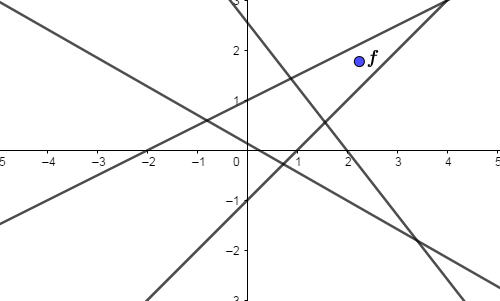
\includegraphics[scale=0.3]{Images/ch3/fig16}
		\caption{} % subcaption
		\label{fig16}
	\end{subfigure}
	\vspace{1em} % here you can insert horizontal or vertical space
	\begin{subfigure}{0.4\textwidth} % width of right subfigure
		\centering
		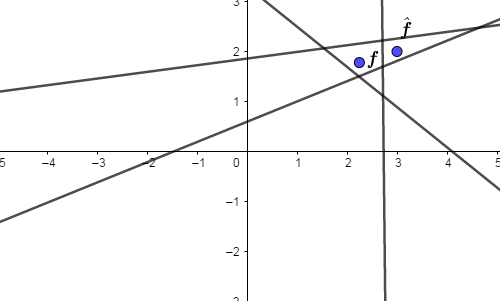
\includegraphics[scale=0.3]{Images/ch3/fig17}
		\caption{} % subcaption
		\label{fig17}
	\end{subfigure}
	\caption{نمایش هندسی تفاوت آستانه‌ی معمولی با آستانه‌ی ابعاد بالا در فضای دو بعدی}
\end{figure}


\subsection{کران خطا}
هدف اصلی از این پایان‌نامه ارائه‌ی یک الگوریتم با آستانه‌گذاری وفقی و مبتنی بر برنامه‌ریزی محدب جهت دست‌یابی به نرخ کاهش نمایی در خطای بازیابی بر حسب تعداد نمونه است. ثابت خواهیم کرد که با استفاده از آستانه‌گذاری ابعاد بالا و الگوریتم‌های نمونه‌برداری و بازیابی مناسب (الگوریتم
\ref{alg:AQ}
و
\ref{alg:AR}
)
قضیه‌ی زیر برقرار است.
\begin{theorem}
\label{thm.main}

الگوریتم‌های نمونه‌برداری و بازیابی وفقی
$ \mathcal{Q} $
و
$ \mathcal{R} $
 ( الگوریتم
\ref{alg:AQ}
و
\ref{alg:AR})
با پارامترهای
$\bm{A}\in \R^{m\times n}$،
$\bm{D}\in \R^{n\times N}$،
$\sigma$،
$r$
و
$L$
 را در نظر بگیرید. همچنین فرض کنید که آستانه‌های مورد نیاز الگوریتم‌ها با استفاده از الگوریتم
$ \Phi $
(الگوریتم
\ref{alg:HDTG})
به  دست آمده باشند. 
فرض کنید
\begin{align}
 m \geq C(r/\sigma+\sigma / r)^{6}(r^{2}/\sigma^2+1)(1/2)^{-6}s \log (N/s) 
\end{align} 
 نمونه از سیگنال
$ \bm{f}\in (\bm{D}^{\ast})^{-1} \Sigma_{s}^{N,\text{eff}} $ 
به صورت
\begin{align}
\label{eq:SignAT}
y_{i}= \text{sign}\left(\langle \bm{a}_{i},\bm{x}\rangle-\bm{\varphi}^{\left(i\right)}\right),
\end{align}

دریافت شده باشد. آنگاه خروجی الگوریتم بازیابی وفقی
$ \mathcal{R} $ 
با احتمال حداقل
\begin{align}
 1-\gamma \exp{(-c^{\prime}m (1/2)^{2} r^2\sigma^2/ (r^2+\sigma^2)^2)} 
\end{align}

در شرط 
\begin{align}
\|\bm{f}-\hat{\bm{f}}\|_{2}\leq r2^{1-L},
\end{align}
 صدق می‌کند.
\end{theorem}
\begin{proof}
یک تعبیر شهودی در 
\ref{proof:IntuitiveMain}
آورده شده است. اثبات ریاضی در پیوست
\ref{Appndx2}
موجود است.
\end{proof}



\subsection{الگوریتم نمونه‌برداری وفقی}
الگوریتم نمونه‌برداری وفقی پیشنهادی به صورت الگوریتم
\ref{alg:AQ}
نشان داده شده است. جهت اجرای این الگوریتم، نیازمند دیکشنری
$ \bm{D} $ 
(دیکشنری که سیگنال
$ \bm{f} $
در آن تنک است.)، ماتریس نمونه‌برداری
$ \bm{A} $
، نمونه‌های خطی
$ \bm{A}\bm{f} $
و یک باند بالای تخمینی از نُرم سیگنال 
$ r $
(
$ \norm{\bm{f}}_{2}\leq r $
) هستیم.
در اولین مرحله از اجرای الگوریتم، مقدار سیگنال تخمینی را صفر در نظر می‌گیریم
($ \hat{\bm{f}}=0 $).
با انتخاب تعداد مراحل تکرار الگوریتم
$ L $
، ماتریس نمونه‌برداری و بردار نمونه‌ها را به 
$ L $
بلوک تقسیم می‌کنیم. در این صورت می‌توانیم فرآیند نمونه‌برداری را آغاز کنیم.


نمونه‌برداری وفقی شامل ۳ مرحله‌ی اصلی است. ابتدا در مرحله‌ی اول،
آستانه‌های ابعاد بالا با استفاده از الگوریتم
\ref{alg:HDTG}
تولید می‌شوند. سپس در مرحله‌ی دوم، بلوک 
$i$ام
از نمونه‌های خطی با آستانه‌ی تولید شده مقایسه می‌گردد و بلوک 
$i$ام
از نمونه‌های تک بیتی تولید می‌شود. در مرحله‌ی بعدی مقدار تخمینی از سیگنال
($\hat{\bm{f}}$)،
با اجرای الگوریتم بازیابی تک-مرحله‌ای بر روی داده‌های بلوک محاسبه می‌گردد. این فرآیند تا مرحله‌ی 
$L$ام
تکرار می‌گردد. جهت افزایش سرعت همگرایی مقدار تخمین زده شده به مقدار اصلی سیگنال، در هر مرحله واریانس بخش تصادفی از آستانه‌های ابعاد بالا، نصف می‌گردد.
در نهایت الگوریتم
\ref{alg:AQ}
مقادیر نمونه‌های تک-بیتی و آستانه را به خروجی می‌فرستد.

\begin{algorithm}
	\caption{$ \mathcal{Q} $: نمونه‌برداری وفقی}
	\label{alg:AQ}
	\begin{algorithmic}[1]
		\renewcommand{\algorithmicrequire}{\textbf{ورودی:}}
		\renewcommand{\algorithmicensure}{\textbf{خروجی:}}
		\REQUIRE دیکشنری $ \bm{D}\in\R^{n\times N} $, ماتریس نمونه‌برداری $ \bm{A}\in\R^{m\times n} $, مشاهدات خطی $ \bm{Af}\in \R^{m} $, تخمین نُرم $ \norm{\bm{f}}_{2}\leq r $, تعداد بلوک‌ها $ L $, $\varDelta$: بازیابی تک مرحله‌ای \eqref{eq:SSR}.
		\ENSURE  نمونه‌های کوانتیزه $ \bm{y} \in \lbrace\pm 1\rbrace^{m} $, آستانه‌ها در ابعاد بالا $ \bm{\varphi} \in \R^{m} $
		\\ \textit{مقدار‌دهی اولیه} : $ \bm{f}_{0}\leftarrow \bm{0} $, $ b = \lfloor\frac{m}{L}\rfloor $, $ \bm{A}^{(i)}\in \R^{b\times m}  $
		\begin{latin}
		\FOR {$i = 1,\cdots,L$}
		\STATE $r_{t}=2^{1-t}r$
		\STATE $\bm{\varphi}^{\left(i\right)}\leftarrow \Phi(\bm{A}^{(i)},b,2^{1-t}r,\bm{f}_{i-1}) $
		\STATE $ \bm{y}^{\left(i\right)} = \text{sign}\left(\bm{A}^{(i)}\bm{f}-\bm{\varphi}^{\left(i\right)}\right)$
		\STATE $ \bm{f}_{i} = \bm{f}_{i-1} + \varDelta\left(\bm{D},\bm{A}^{(i)},\bm{y}^{\left(i\right)},\bm{\varphi}^{\left(i\right)},\bm{r}_{t}\right) $
		\ENDFOR
		\end{latin}
	\end{algorithmic} 
\end{algorithm}




\subsection{الگوریتم بازیابی وفقی}
در فرآیند بازیابی (الگوریتم
\ref{alg:AR})
نیازمند دیکشنری
$ \bm{D} $
ماتریس نمونه‌برداری
$ \bm{A} $
بردار نمونه‌های تک بیتی
$ \bm{y} $
بردار آستانه‌های ابعاد بالا
$ \bm{\varphi} $
و یک باند بالای تخمینی از نُرم سیگنال
$ r $
، هستیم. پس از اعمال مقادیر فوق به عنوان ورودی الگوریتم
\ref{alg:AR}
،‌ می‌توان الگوریتم را اجرا نمود. در روند اجرای بازیابی وفقی، با تقسیم بردار اندازه‌گیری،‌ نمونه‌ها و آستانه‌ها به 
$ L $
بلوک آغاز می‌گردد. در هر مرحله از اجرای الگوریتم، تنها الگوریتم بازیابی تک مرحله‌ای به ازای ورودی‌های مختلف اجرا می‌گردد.



\begin{algorithm}
	\caption{$ \mathcal{R} $: بازیابی وفقی}
	\label{alg:AR}
	\begin{algorithmic}[1]
		\renewcommand{\algorithmicrequire}{\textbf{ورودی:}}
		\renewcommand{\algorithmicensure}{\textbf{خروجی:}}
		\REQUIRE دیکشنری $ \bm{D}\in\R^{n\times N} $, ماتریس نمونه‌برداری $ \bm{A}\in\R^{m\times n} $, نمونه‌های کوانتیزه $ \bm{y} \in \lbrace\pm 1\rbrace^{m} $, آستانه‌ها در ابعاد بالا $ \bm{\varphi}\in\R^{m} $, تخمین نُرم $ \norm{\bm{f}}_{2}\leq r $, تعداد بلوک‌ها $ L $، $\varDelta$: بازیابی تک مرحله‌ای \eqref{eq:SSR}.
		\ENSURE  تخمین سیگنال $ \hat{\bm{f}}\in \R^{n} $.
		\\ \textit{مقداردهی اولیه} :  $ b = \lfloor\frac{m}{L}\rfloor $, $ \bm{A}^{(i)}\in \R^{b\times m}$, $ \bm{y}^{\left(i\right)} \lbrace\pm 1\rbrace^{b}$, $\bm{\varphi}^{\left(i\right)}\in \R^{b} $
		\begin{latin}
		\FOR {$i = 1,\cdots,L$}
		\STATE $ \bm{f}_{i} =\bm{f}_{i-1}+ \varDelta\left(\bm{D},\bm{A}^{(i)},\bm{y}^{\left(i\right)},\bm{\varphi}^{\left(i\right)},\bm{r}_{t}\right) $ 
		\ENDFOR
		\end{latin}
	\end{algorithmic} 
\end{algorithm}


نکته‌ی قابل توجه در الگوریتم بازیابی وفقی تکرار عملیات‌ها است. اگر دوباره به الگوریتم نمونه‌برداری وفقی نگاه کنیم، متوجه می‌شویم که الگوریتم 
\ref{alg:AR}
یک بخش از الگوریتم 
\ref{alg:AQ}
است. برتری الگوریتم بازیابی وفقی این است که نیاز به بردار نمونه‌های خطی
($\bm{A}\bm{f}$)
 ندارد و تنها با استفاده از نمونه‌های تک بیتی می‌تواند بازیابی سیگنال را انجام دهد. این موضوع، در صورتی که بین محل نمونه‌برداری و بازیابی فاصله باشد کاربرد خواهد داشت. به عبارت دیگر از الگوریتم نمونه‌برداری وفقی می‌توان به عنوان یک کدگذار
 \LTRfootnote{Encoder}
  و از الگوریتم بازیابی وفقی به عنوان کدگشا
 \LTRfootnote{Decoder}
 استفاده نمود. در این حالت با توجه به اینکه نمونه‌ها تک بیتی هستند حجم داده‌ی مورد نیاز جهت انتقال به شدت کاهش خواهد یافت.

\subsection{تعبیر شهودی قضیه‌ی ۹}
\label{proof:IntuitiveMain}
در این بخش، اثبات شهودی برای قضیه‌ی
\ref{thm.main}
آورده شده است. قبل از شروع اثبات، بهتر است که یک مرور سریع بر صورت قضیه داشته باشیم.

به صورت خلاصه در این قضیه، ما الگوریتم بازیابی تک مرحله‌ای را برای مقدار لغزش و مرکز مختلف، طی 
$L$
مرحله اجرا می‌کنیم. جهت اثبات این قضیه از نتایج حسگری فشرده‌ی تک بیتی سنتی استفاده شده است. تصویر بر نیم‌کره (تعریف
\ref{defn:HP}
)
در اینجا نقش پل بین حسگری فشرده تک بیتی سنتی و نتایج ارائه شده در این پایان‌نامه را بازی می‌کند.

یک نیم کره با شعاع 
$\sigma$
و مرکز مبدا مختصات در نظر بگیرید. این نیم کره در نقطه‌ی 
$ [\bm{0}^{T}~|~\sigma]^{T}\in \R^{n+1} $
به فضای سیگنال
$ \bm{f} $ 
مماس است. به خاطر آورید که هر سطر از ماتریس 
$\bm{A}$
مشخص کننده‌ی بردار نرمال یک ابرصفحه در فضای
$ \R^{n} $
است. هر کدام از این ابرصفحه‌ها را می‌توان به صورت یک ابرصفحه‌ی دیگر که از مبدا مختصات در فضای 
$ \R^{n+1} $
عبور می‌کند در نظر گرفت. در چنین شرایطی، پس از تصویر نمودن فضای سیگنال بر نیم‌کره، فضای جدید برابر با نیمه‌ی بالایی 
 $ \sigma S^{n} $
است که توسط تعداد مشخصی از ابرصفحه‌ها برش داده شده است.

همان‌گونه که در قسمت‌های قبلی بیان گردید،  الگوریتم با یک مقدار تخمین از نُرم سیگنال
$ \norm{\bm{f}}_{2} $
آغاز می‌گردد. تعبیر هندسی این انتخاب این است که در ابتدای کار، نقاطی که در فاصله‌ی دورتر نسبت به نقطه‌ی تماس قرار دارند، به نقاط مناسب از نیم‌کره تصویر می‌گردند. این موضوع باعث می‌شود که پاسخ تقریبی به دست آمده در مراحل اولیه از دقت مناسب برخوردار باشد. در هر مرحله از الگوریتم نمونه‌برداری، با استفاده از الگوریتم آستانه‌گذاری ابعاد بالا،(الگوریتم
\ref{alg:HDTG})
نقطه‌ی تماس نیم‌کره با فضای سیگنال
$ \bm{f} $ 
به محل سیگنال تخمین زده شده جابجا می‌شود و با کاهش شعاع نیم‌کره که معادل با کاهش واریانس مقادیر لغزش است، با دقت بیشتری نمونه‌های جدید را اخذ می‌کند. این فرآیند منجر به نمونه‌برداری با کیفیت بهتر می‌شود و به همین دلیل خطای بازیابی کاهش می‌یابد.














